\documentclass[main]{subfiles}


\title[AutoML in the Age of Foundation Models]{AutoML in the Age of Foundation Models}
\subtitle{Next Level AutoML by Agentic AI}
\author[Marius Lindauer]{Marius Lindauer}
\date{}

\titlebackground*{images/AutoML_Agentic}

%\institute{}
%\date{}

\begin{document}
	
	\maketitle
	

%----------------------------------------------------------------------
%----------------------------------------------------------------------
\begin{frame}{Motivation: The Shift to Agentic AutoML}
\begin{itemize}
    \item Traditional AutoML systems require manual configuration, rigid data formatting, and heavy domain expertise, limiting their accessibility.
    \item Current Large Language Model (LLM) agents struggle with end-to-end ML complexity; they rely too heavily on inherent parametric knowledge (leading to outdated or overly simple model choices) and lack targeted, component-specific debugging.
    \item \textbf{General Idea:} Leverage multi-agent architectures to autonomously perceive data, plan pipelines, generate executable code, and verify/refine solutions iteratively. \end{itemize}
\end{frame}

\begin{frame}{Core Commonalities Across Frameworks}
\begin{itemize}
    \item \textbf{Multi-Agent Orchestration:} Decomposition of the ML pipeline into specialized roles (e.g., Data/Perception Agents, Coder/Implementation Agents, Planning Agents, and Verification Agents).     \item \textbf{Iterative Execution \& Feedback:} Conceptualizing machine learning engineering as a code optimization problem to find the optimal script $s^* \in \arg\min_{s \in \mathcal{S}} \cost(s)$ given a metric $\cost$.
    \item \textbf{External Knowledge Integration:} Mitigating LLM hallucination by grounding the generation process in retrieved external knowledge rather than relying purely on internal model weights.
\end{itemize}
\end{frame}

\begin{frame}{AutoML-Agent: Retrieval-Augmented Planning\\ \liturl{Trirat et al. 2024}{https://arxiv.org/abs/2410.02958}}
\begin{itemize}
    \item \textbf{Objective:} Address complex inter-dependencies in full-pipeline AutoML without the high computational cost of training-based model search.
    \item \textbf{Retrieval-Augmented Planning (RAP):} Generates multiple diverse end-to-end plans via API calls prior to execution.
    \item \textbf{Prompting-Based Plan Execution:} Decomposes plans into sub-tasks. Simulates model search using pseudo-data analysis without actual execution overhead.
    \item \textbf{Multi-Stage Verification:} Incorporates strict request, execution, and implementation verification steps.
\end{itemize}
\end{frame}

\begin{frame}{AutoML-Agent: Retrieval-Augmented Planning\\ \liturl{Trirat et al. 2024}{https://arxiv.org/abs/2410.02958}}

\centering
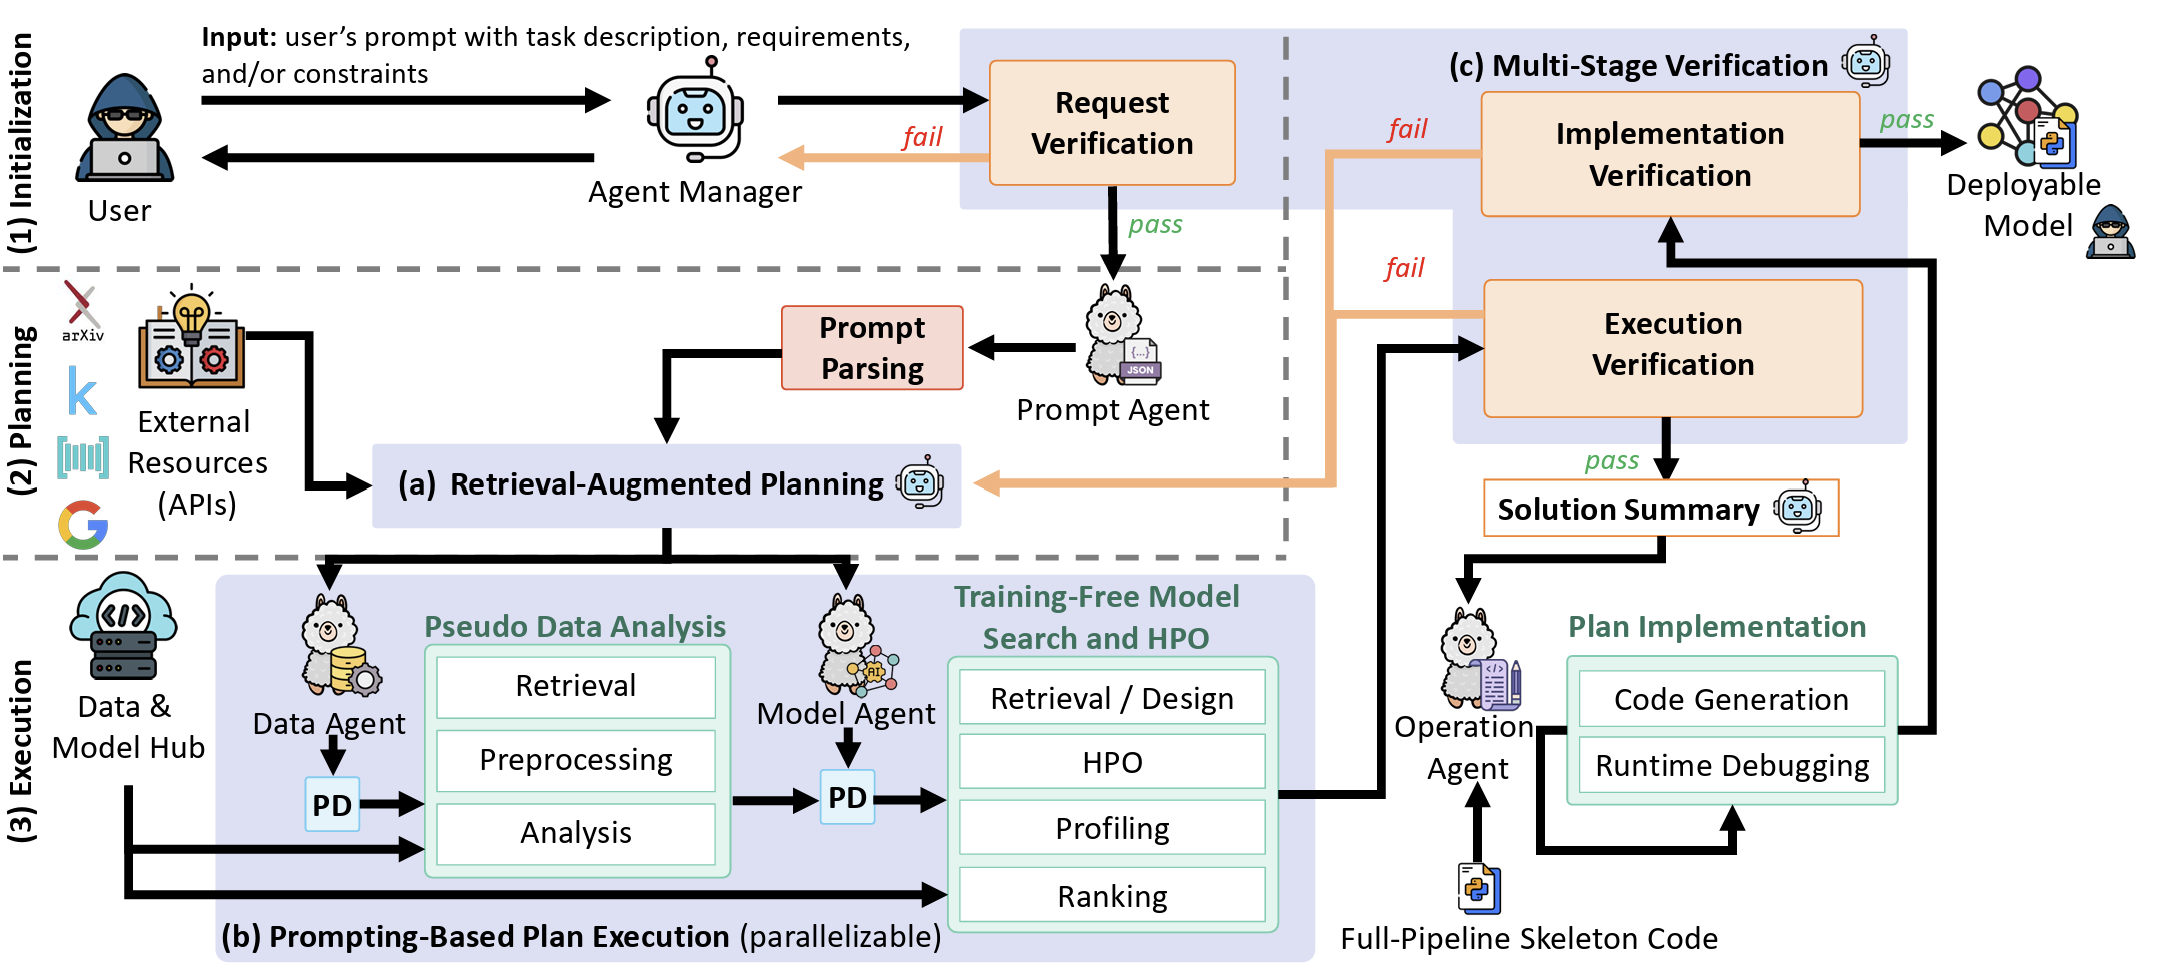
\includegraphics[width=0.9\textwidth]{images/automl_agent.png}

\end{frame}

\begin{frame}{MLE-STAR: Targeted Refinement \& Ensembling\\ \liturl{Nam et al. 2025}{https://arxiv.org/pdf/2506.15692}}
\begin{itemize}
    \item \textbf{Objective:} Overcome coarse, whole-script exploration by targeting specific pipeline components for deep refinement.
    \item \textbf{Targeted Code Block Extraction:} Uses ablation studies to find the most impactful code block.
    \item \textbf{Code Block Refinement:} Refines \textit{only} the extracted block and replaces it directly in the script.
    \item \textbf{Agentic Ensembling:} Rather than simple majority voting, a specialized planner proposes and iterates dynamic ensemble strategies.
\end{itemize}
\end{frame}

\begin{frame}{MLE-STAR: Targeted Refinement \& Ensembling\\ \liturl{Nam et al. 2025}{https://arxiv.org/pdf/2506.15692}}

\centering
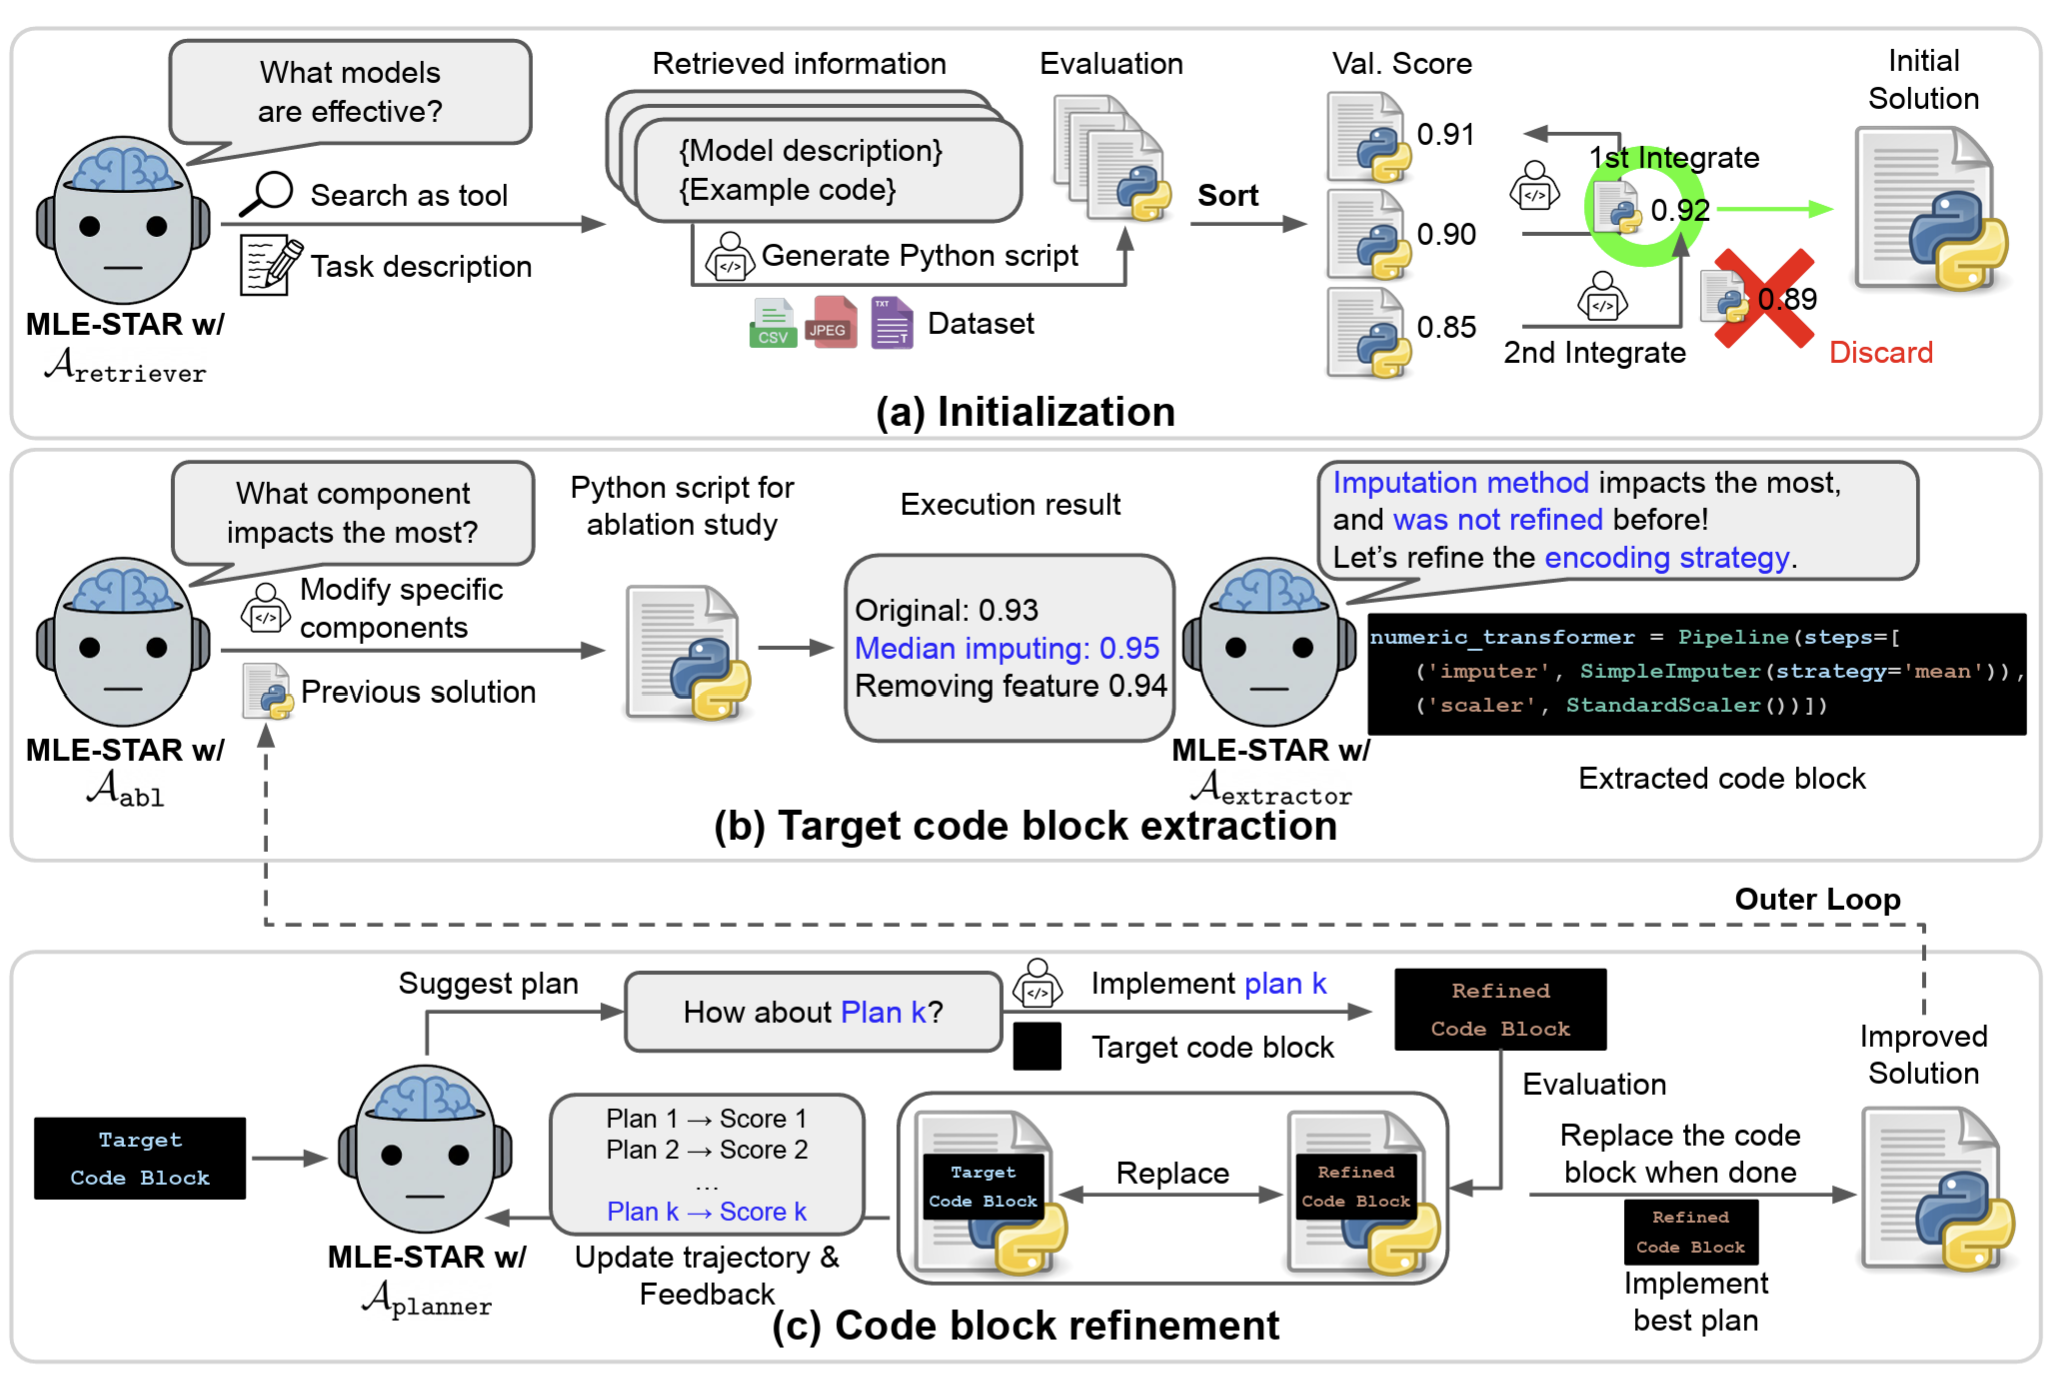
\includegraphics[width=.65\textwidth]{images/mle_star.png}

\end{frame}

\begin{frame}{MLZero: Cognitive Perception and Dual Memory\\ \liturl{Fang et al. 2025}{https://arxiv.org/pdf/2505.13941}}
\begin{itemize}
    \item \textbf{Objective:} Achieve zero human intervention across diverse, raw multimodal data.
    \item \textbf{Cognitive Perception:} Autonomously extracts perceptual context and library choice.
    \item \textbf{Structured Memories:}
    \begin{itemize}
        \item \textit{Semantic Memory:} Condenses library documentation into searchable knowledge.
        \item \textit{Episodic Memory:} Records chronological execution logs and errors to provide targeted debugging context.
    \end{itemize}
    \item \textbf{Iterative Coding:} Code generation continuously integrates these memories.
\end{itemize}
\end{frame}


% \begin{frame}{Specialized Algorithmic Differences}
% \begin{itemize}
%     \item \textbf{Exploration Strategy:} 
%     \begin{itemize}
%         \item \textit{AutoML-Agent:} Breadth-first pseudo-execution (training-free) via prompt simulation to minimize search cost.
%         \item \textit{MLE-STAR:} Nested loops (Outer loop targets a code block via ablation; Inner loop explores $K$ plan refinements on that specific block).
%     \end{itemize}
%     \item \textbf{Memory vs. Search:}
%     \begin{itemize}
%         \item \textit{MLZero:} Relies heavily on offline-indexed \textit{Semantic Memory} (condensed library documentation).
%         \item \textit{MLE-STAR \& AutoML-Agent:} Actively use \textit{Web Search / APIs} dynamically during the planning phase to find up-to-date, state-of-the-art models.
%     \end{itemize}
%     \item \textbf{Data Handling:} MLZero handles entirely raw files with a dedicated perception module, while others employ robust pre-execution checks (e.g., MLE-STAR's Data Leakage Checker).
% \end{itemize}
% \end{frame}

\begin{frame}{Summary}
\begin{itemize}
    \item \textbf{Modularity Over Monoliths:} Complex, open-ended tasks require decomposing the problem space into discrete components managed by highly specialized agents (e.g., separating perception, coding, and ensembling).
    \item \textbf{Grounding Trumps Parametric Knowledge:} Even advanced LLMs hallucinate syntax or default to outdated methods. Integrating external knowledge is mandatory for state-of-the-art performance.     \item \textbf{Feedback-Driven Refinement:} The most effective autonomous systems implement explicit self-reflection—whether through simulated execution, episodic execution history, or targeted code ablations—shifting from "one-shot generation" to "iterative optimization."
\end{itemize}
\end{frame}
%-----------------------------------------------------------------------



\end{document}

